% 通用样式文件 - 统一所有文档的样式

% 目录样式设置 - 干净简洁,无边框,优化编号
% 使用基本 LaTeX 命令美化目录
\makeatletter
\renewcommand\@dotsep{2}
% 优化编号格式:减少缩进,使编号更紧凑
\renewcommand\l@section{\@dottedtocline{1}{0em}{1.2em}}
\renewcommand\l@subsection{\@dottedtocline{2}{1.2em}{1.8em}}
\renewcommand\l@subsubsection{\@dottedtocline{3}{3em}{2.2em}}
% 设置目录深度为3,显示到subsubsection级别
\setcounter{tocdepth}{3}
\makeatother

% 超链接设置 - 目录链接无颜色框
\hypersetup{
    colorlinks=true,
    linkcolor=black,          % 目录链接为黑色
    filecolor=black,
    urlcolor=blue,
    citecolor=black,
    pdfstartview=FitH,
    pdfborder={0 0 0},        % 无边框
    linkbordercolor={0 0 0},  % 链接边框颜色为黑色(不可见)
    pdfborderstyle={/S/U},    % 无边框样式
}

% 页眉页脚设置(在文档中重新定义)
\usepackage{fancyhdr}
% 注意:每个文档需要在导入 common_style.tex 后设置自己的页眉页脚

% 章节格式 - 简洁美观(使用基本命令)
\makeatletter
\renewcommand\section{\@startsection {section}{1}{\z@}%
                                   {-3.5ex \@plus -1ex \@minus -.2ex}%
                                   {2.3ex \@plus.2ex}%
                                   {\normalfont\Large\bfseries}}
\renewcommand\subsection{\@startsection{subsection}{2}{\z@}%
                                     {-3.25ex\@plus -1ex \@minus -.2ex}%
                                     {1.5ex \@plus .2ex}%
                                     {\normalfont\large\bfseries}}
\renewcommand\subsubsection{\@startsection{subsubsection}{3}{\z@}%
                                     {-3.25ex\@plus -1ex \@minus -.2ex}%
                                     {1.5ex \@plus .2ex}%
                                     {\normalfont\normalsize\bfseries}}
\makeatother

% 代码样式设置 - 简洁干净,无背景色
\definecolor{codegray}{rgb}{0.5,0.5,0.5}
\definecolor{keywordblue}{rgb}{0,0,0.8}
\definecolor{stringred}{rgb}{0.3,0.3,0.3}
\definecolor{commentgreen}{rgb}{0,0.5,0}

\lstdefinestyle{pythonstyle}{
    language=Python,
    % 无背景色 - 使用白色背景,与文档背景一致
    commentstyle=\color{commentgreen},      % 注释不用斜体
    keywordstyle=\color{keywordblue}\bfseries,
    stringstyle=\color{stringred},
    basicstyle=\ttfamily\small,
    breakatwhitespace=false,
    breaklines=true,
    captionpos=b,
    keepspaces=true,
    numbers=none,                           % 不显示行号
    showspaces=false,
    showstringspaces=false,
    showtabs=false,
    tabsize=4,
    frame=single,                          % 保留边框,但更简洁
    rulecolor=\color{black},
    framerule=0.5pt,                       % 细边框
    framexleftmargin=8pt,                  % 左边距(代码与左边框的距离)
    framexrightmargin=8pt,                 % 右边距(代码与右边框的距离)
    framextopmargin=6pt,                   % 上边距(代码与上边框的距离)
    framexbottommargin=6pt,                % 下边距(代码与下边框的距离)
    morekeywords={import,from,as,class,def,return,yield,lambda,if,elif,else,for,while,break,continue,pass,try,except,finally,raise,assert,with,del,global,nonlocal,and,or,not,in,is},
    identifierstyle=\color{black},
}

\lstset{style=pythonstyle}

% 封面宏定义
\newcommand{\makecover}[5]{%
    \newpage
    \thispagestyle{empty}
    \vspace*{1.5cm}
    \begin{center}
        \vspace{2cm}
        {\fontsize{48}{58}\selectfont\bfseries #1}\\[0.8cm]
        \vspace{1.5cm}
        {\Large #2}\\[0.4cm]
        \vspace{1.5cm}
        {\large #3}\\[1.5cm]
        
        % 神经网络图 - 紧凑版本,无标签
        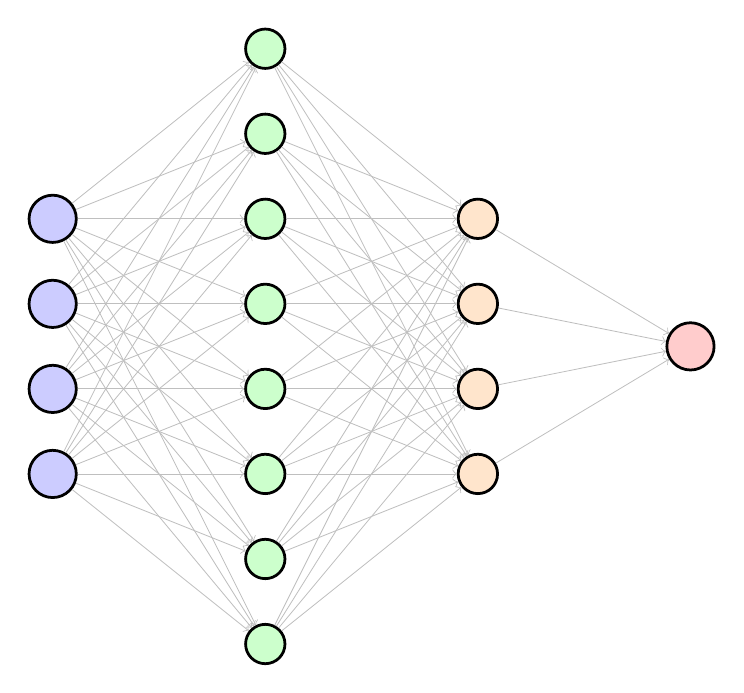
\begin{tikzpicture}[scale=0.9]
        % 定义神经元间距
        \def\spacing{1.2}
        
        % 输入层 - 4个神经元,关于横轴对称
        \node[circle, draw, minimum size=0.6cm, fill=blue!20, line width=1pt] (x1) at (0, -1.8) {};
        \node[circle, draw, minimum size=0.6cm, fill=blue!20, line width=1pt] (x2) at (0, -0.6) {};
        \node[circle, draw, minimum size=0.6cm, fill=blue!20, line width=1pt] (x3) at (0, 0.6) {};
        \node[circle, draw, minimum size=0.6cm, fill=blue!20, line width=1pt] (x4) at (0, 1.8) {};
        
        % 隐藏层1 - 8个神经元,关于横轴对称
        \node[circle, draw, minimum size=0.5cm, fill=green!20, line width=1pt] (h11) at (3, -4.2) {};
        \node[circle, draw, minimum size=0.5cm, fill=green!20, line width=1pt] (h12) at (3, -3.0) {};
        \node[circle, draw, minimum size=0.5cm, fill=green!20, line width=1pt] (h13) at (3, -1.8) {};
        \node[circle, draw, minimum size=0.5cm, fill=green!20, line width=1pt] (h14) at (3, -0.6) {};
        \node[circle, draw, minimum size=0.5cm, fill=green!20, line width=1pt] (h15) at (3, 0.6) {};
        \node[circle, draw, minimum size=0.5cm, fill=green!20, line width=1pt] (h16) at (3, 1.8) {};
        \node[circle, draw, minimum size=0.5cm, fill=green!20, line width=1pt] (h17) at (3, 3.0) {};
        \node[circle, draw, minimum size=0.5cm, fill=green!20, line width=1pt] (h18) at (3, 4.2) {};
        
        % 隐藏层2 - 4个神经元,关于横轴对称
        \node[circle, draw, minimum size=0.5cm, fill=orange!20, line width=1pt] (h21) at (6, -1.8) {};
        \node[circle, draw, minimum size=0.5cm, fill=orange!20, line width=1pt] (h22) at (6, -0.6) {};
        \node[circle, draw, minimum size=0.5cm, fill=orange!20, line width=1pt] (h23) at (6, 0.6) {};
        \node[circle, draw, minimum size=0.5cm, fill=orange!20, line width=1pt] (h24) at (6, 1.8) {};
        
        % 输出层 - 1个神经元,在横轴上
        \node[circle, draw, minimum size=0.6cm, fill=red!20, line width=1pt] (y) at (9, 0) {};
        
        % 输入层到隐藏层1的连接
        \foreach \i in {1,...,4}
            \foreach \j in {1,...,8}
                \draw[->, gray!50, line width=0.3pt] (x\i) -- (h1\j);
        
        % 隐藏层1到隐藏层2的连接
        \foreach \i in {1,...,8}
            \foreach \j in {1,...,4}
                \draw[->, gray!50, line width=0.3pt] (h1\i) -- (h2\j);
        
        % 隐藏层2到输出层的连接
        \foreach \i in {1,...,4}
            \draw[->, gray!50, line width=0.3pt] (h2\i) -- (y);
        \end{tikzpicture}
        
        \vfill
        \vspace{2cm}
        {\normalsize #5}
        \vspace{1.5cm}
    \end{center}
    \newpage
}

